\documentclass[unicode,11pt,a4paper,oneside,numbers=endperiod,openany]{scrartcl}

\usepackage{ifthen}
\usepackage[utf8]{inputenc}
\usepackage{graphics}
\usepackage{graphicx}
\usepackage{hyperref}
%%%%%%%%%%%%%%%%%%%%% Added Packages: %%%%%%%%%%%%%%%%%%%%%%%%%%%%%%%%%%
\usepackage{amsmath}
\usepackage{float}

\usepackage[dvipsnames]{xcolor}
\usepackage{fancyvrb}

\usepackage{subcaption}
\usepackage{ifthen}
\usepackage{listings}



% redefine \VerbatimInput
\RecustomVerbatimCommand{\VerbatimInput}{VerbatimInput}%
{fontsize=\footnotesize,
 %
 frame=lines,  % top and bottom rule only
 framesep=2em, % separation between frame and text
 rulecolor=\color{Gray},
 %
%  label=\fbox{\color{Black}slurm-euler\_phase\_1.txt},
%  labelposition=topline,
 %
 commandchars=\|\(\), % escape character and argument delimiters for
                      % commands within the verbatim
 commentchar=*        % comment character
}

% \newcommand{\myInputFile}{slurm-euler_phase_1.txt} % Set the default input file
% \newboolean{isPhaseOne}
% \setboolean{isPhaseOne}{true} % Set to false for phase 2

% % Redefine \VerbatimInput
% \RecustomVerbatimCommand{\VerbatimInput}{VerbatimInput}%
% {
%     fontsize=\footnotesize,
%     frame=lines,  % top and bottom rule only
%     framesep=2em, % separation between frame and text
%     rulecolor=\color{Gray},
%     label=\fbox{\ifthenelse{\boolean{isPhaseOne}}{\color{Black}slurm-euler\_phase\_1.txt}{\color{Black}slurm-euler\_phase\_2.txt}},
%     labelposition=topline,
%     commandchars=\|\(\), % escape character and argument delimiters for
%                           % commands within the verbatim
%     commentchar=*        % comment character
% }
%%%%%%%%%%%%%%%%%%%%%%%%%%%%%%%%%%%%%%%%%%%%%%%%%%%%%%%%%%%%%%%%%%%%%%%

\pagestyle{plain}
\voffset -5mm
\oddsidemargin  0mm
\evensidemargin -11mm
\marginparwidth 2cm
\marginparsep 0pt
\topmargin 0mm
\headheight 0pt
\headsep 0pt
\topskip 0pt        
\textheight 255mm
\textwidth 165mm

\newcommand{\duedate} {}
\newcommand{\setduedate}[1]{%
\renewcommand\duedate {Due date:~ #1}}
\newcommand\isassignment {false}
\newcommand{\setassignment}{\renewcommand\isassignment {true}}
\newcommand{\ifassignment}[1]{\ifthenelse{\boolean{\isassignment}}{#1}{}}
\newcommand{\ifnotassignment}[1]{\ifthenelse{\boolean{\isassignment}}{}{#1}}

\newcommand{\assignmentpolicy}{
\begin{table}[h]
\begin{center}
\scalebox{0.8} {%
\begin{tabular}{|p{0.02cm}p{16cm}|}
\hline
&\\
\multicolumn{2}{|c|}{\Large\textbf{HPC Lab for CSE 2024 ---  Submission Instructions}}\\
\multicolumn{2}{|c|}{\large\textbf{(Please, notice that following instructions are mandatory: }}\\
\multicolumn{2}{|c|}{\large\textbf{submissions that don't comply with, won't be considered)}}\\
&\\
\textbullet & Assignments must be submitted to \href{https://moodle-app2.let.ethz.ch/course/view.php?id=22516}{Moodle} (i.e. in electronic format).\\
\textbullet & Provide both executable package and sources (e.g. C/C++ files, Matlab). 
If you are using libraries, please add them in the file. Sources must be organized in directories called:\\
\multicolumn{2}{|c|}{\textit{Project\_number\_lastname\_firstname}}\\
& and  the  file must be called:\\
\multicolumn{2}{|c|}{\textit{project\_number\_lastname\_firstname.zip}}\\
\multicolumn{2}{|c|}{\textit{project\_number\_lastname\_firstname.pdf}}\\
\textbullet &  The TAs will grade your project by reviewing your project write-up, and looking at the implementation 
                 you attempted, and benchmarking your code's performance.\\

\textbullet & You are allowed to discuss all questions with anyone you like; however: (i) your submission must list anyone you discussed problems with and (ii) you must write up your submission independently.\\
\hline
\end{tabular}
}
\end{center}
\end{table}
}
\newcommand{\punkte}[1]{\hspace{1ex}\emph{\mdseries\hfill(#1~\ifcase#1{Points}\or{Points}\else{Points}\fi)}}


\newcommand\serieheader[6]{
\thispagestyle{empty}%
\begin{flushleft}

\includegraphics[width=0.4\textwidth]{Images/ETHlogo_13}
\end{flushleft}
  \noindent%
  {\large\ignorespaces{\textbf{#1}}\hspace{\fill}\ignorespaces{ \textbf{#2}}}\\ \\%
  {\large\ignorespaces #3 \hspace{\fill}\ignorespaces #4}\\
  \noindent%
  \bigskip
  \hrule\par\bigskip\noindent%
  \bigskip {\ignorespaces {\Large{\textbf{#5}}}
  \hspace{\fill}\ignorespaces \large \ifthenelse{\boolean{\isassignment}}{\duedate}{#6}}
  \hrule\par\bigskip\noindent%  \linebreak
 }

\makeatletter
\def\enumerateMod{\ifnum \@enumdepth >3 \@toodeep\else
      \advance\@enumdepth \@ne
      \edef\@enumctr{enum\romannumeral\the\@enumdepth}\list
      {\csname label\@enumctr\endcsname}{\usecounter
        {\@enumctr}%%%? the following differs from "enumerate"
	\topsep0pt%
	\partopsep0pt%
	\itemsep0pt%
	\def\makelabel##1{\hss\llap{##1}}}\fi}
\let\endenumerateMod =\endlist
\makeatother




\usepackage{textcomp}






\begin{document}


\setassignment
\setduedate{11 March 2024, 23:59}

\serieheader{High-Performance Computing Lab for CSE}{2024}
            {Student: Yannick Ramic}
            {Discussed with: Patrick Dowd, Carla Zurita, Arsh Kumbhat}{Solution for Project 1}{}
\newline

\assignmentpolicy

\section{Euler warm-up [10 points]}
This answers come from the documentation website, hence I won't cite anything properly.
\subsection{What is the module system and how do you use it?}
While working on the cluster it's necessary to use software or work with programming
languages like C++ or Python. To make use of the cluster and use it's potential to work
with accelerated GPU and CPU, these dependencies need to be actually installed on the 
cluster. Thus, to configure the desired environment with a prefered software version, the
cluster makes use of modules. For the EULER cluster, two types of modules exist. LMOD
modules, which use a hierarchy of modules with three layers (Core -, Compiler - and MPI layer,
according to the illustration on the documentation webpage). On the other hand, environment
modules have the advantage to make use of pre-installed dependencies by updating the
desired software stock. More important information, users are able to install additional
applications in their home directory, also there are useful commands to check whether a 
dependency is installed.
\subsection{What is SLURM and its intended function?}
SLURM is a workload manager for the management of compute jobs on high-performance computing 
clusters. It's important to know that 
users can solely use the cluster ressources through the batch system. During the lecture it
was made clear that for each job submitted we need ro make a request at the cluster,
which is done by the described batch system! Thus a job submission command consists of three
parts:
\begin{enumerate}
    \item sbatch (SLURM submit command)
    \item SLURM options (requesting resources and job-related options)
    \item Job (computing job to be submitted)
\end{enumerate}
To summarize, the intended function is to efficiently delegate and utilize computing resources.
Further information about how to submit a job, a parallel job, a GPU job, as well as, how to 
monitor a job and see the job output can be found on the EULER cluster documentation online!
\subsection{Write a simple "Hello World" C/C++ program which prints the host name of the machine
on which the program is running.}
You can find the corresponding C++ file under the name \texttt{hello\_world.cpp}.
\subsection{Write a batch script which runs your program on one node. The batch script should
be able to target nodes with specific CPUs}
The resulting files are \texttt{slurm\_job\_one-49284262.out} and \texttt{slurm\_job\_one-49284262.err}.
\subsection{Write another batch script which runs your program on two nodes}
The resulting files are \texttt{slurm\_job\_two-49289041.out} and \texttt{slurm\_job\_two-49289041.err}.

\section{Performance characteristics [50 points]}

\subsection{Peak performance}

This task requires the computation of the core, CPU, node and cluster peak performance for the Euler VII (phase 1 and 2) nodes. Relevant
information from the provided webpages can be found summarized in table \ref{tab:CPU_par}. Also from the exercise sheet we get the following
formulas for calculating the cluster peak perfromances:
\begin{align*}
    P_{core} &= n_{super} \cdot n_{FMA} \cdot n_{SIMD} \cdot f \\
    P_{CPU} &= n_{core} \cdot P_{core} \\
    P_{node} &= n_{sockets} \cdot P_{CPU} \\
    P_{cluster} &= n_{node} \cdot P_{node}
\end{align*}

In addition I want to note a few things. The value from $n_{SIMD}$ comes from the fact that both AMD processors support AVX2 SIMD instructions
with 256-bit wide vector registers. Since we are dealing with double-precision FP numbers the size of the vector register needs to be divided
by 64 bits, this will result in the $n_{SIMD}$ value. Also from the given optimization manual for each processor unit we have to get the information
if FMA (Floating Multiply Add) is provided. Since both processors support FMA, the fused multiply-add factor $n_{FMA}$ = 2 otherwise it would just be 1
and the multiplication and addition can't happen in a single operation. f is the base clock frequency and key characteristic of each CPU. In addition,
it should be mentioned that a good approximation for the duration of one clock cycle is given by 1/f. This number helps measuring the execution time
of instructions. 
\begin{table}[h]
    \centering
    \begin{tabular}{lrr}
      \hline
      Parameter & Phase 1 & Phase 2 \\
      \hline
      $n_{nodes}$ & 292 & 248\\
      $n_{sockets}$ & 2 & 2\\
      $n_{cores}$ & 64 & 64\\
      $n_{super}$ & 2 & 2\\
      $n_{FMA}$ & 2 & 2\\
      $n_{SIMD}$ & 4 & 4\\
      f in [GHz] & 2,6 & 2.45\\
      \hline
    \end{tabular}
    \caption{CPU Parameter}
    \label{tab:CPU_par}
  \end{table}

From table \ref{tab:CPU_par} we get the following theoretical values for the Euler VII Phase 1:
\begin{align*}
    P_{core} &= 2 \cdot 2 \cdot 4 \cdot 2.6 GHz = 41.6 GFlops/s \\
    P_{CPU} &= 64 \cdot 41.6 GFlops/s = 2662.4 GFlops/s \\
    P_{node} &= 2 \cdot 2662.4 GFlops/s = 5324.8 GFlopts/s \\
    P_{Euler VII}^{(1)} &= 292 \cdot 5324.8 GFlops/s = 1554.8416 TFlops/s
\end{align*}

Analog for the Euler VII Phase 2 these are the results:
\begin{align*}
    P_{core} &= 2 \cdot 2 \cdot 4 \cdot 2.45 GHz = 39.2 GFlops/s \\
    P_{CPU} &= 64 \cdot 39.2 GFlops/s = 2508.8 GFlops/s \\
    P_{node} &= 2 \cdot 2508.8 GFlops/s = 5017.6 GFlopts/s \\
    P_{Euler VII}^{(2)} &= 248 \cdot 5017.6 GFlops/s = 1244.3648 TFlops/s
\end{align*}

\subsection{Memory Hierarchies}

The result of the command lscpu can be summarized in the following table:

\begin{table}[h]
    \centering
    \begin{tabular}{|l|l|}
      \hline
      \textbf{Information} & \textbf{Resulting Output} \\
      \hline
      Architecture & x86\_64 \\
      CPU op-mode(s) & 32-bit, 64-bit \\
      Byte Order & Little Endian \\
      CPU(s) & 4 \\
      On-line CPU(s) list & 0-3 \\
      Thread(s) per core & 1 \\
      Core(s) per socket & 4 \\
      Socket(s) & 1 \\
      NUMA node(s) & 1 \\
      Vendor ID & GenuineIntel \\
      CPU family & 6 \\
      Model & 71 \\
      Model name & Intel(R) Xeon(R) CPU E3-1284L v4 @ 2.90GHz \\
      Stepping & 1 \\
      CPU MHz & 1403.802 \\
      CPU max MHz & 3800.0000 \\
      CPU min MHz & 800.0000 \\
      BogoMIPS & 5799.77 \\
      Virtualization & VT-x \\
      L1d cache & 32K \\
      L1i cache & 32K \\
      L2 cache & 256K \\
      L3 cache & 6144K \\
      L4 cache & 131072K \\
      NUMA node0 CPU(s) & 0-3 \\
      \hline
    \end{tabular}
    \caption{Result of the command \$ lscpu}
    \label{tab:lscpu}
\end{table}

The total available main memory with the command cat /proc/meminfo 
is:
\begin{align*}
    MemoryTotal = 32871604 kB
\end{align*}
Now we want to gain information about the memory hierarchy, which can be achieved by the
following command \$ hwloc-ls --whole-system --no-io the result is the same as depicted in the exercise sheet.
In the end I want to obtain the figure and all necessary commands are described as well in the exercise sheet.
The resulting hierarchy is depicted in figure

\begin{figure}[H]
    \centering
    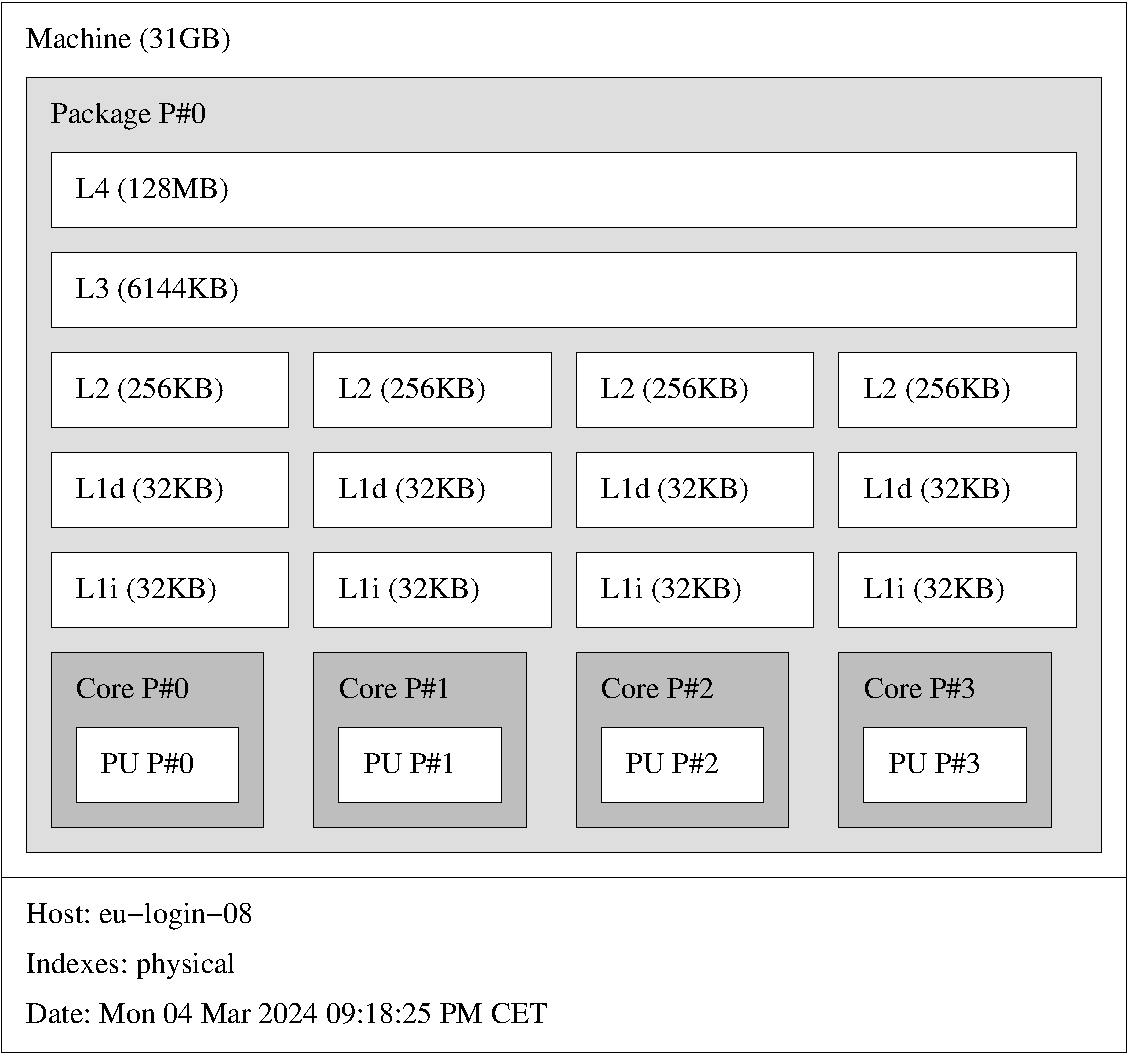
\includegraphics[width=\textwidth]{Images/XEON_E3-1284L.pdf}
    \caption{Schematic of an Euler login node with an Intel(R) Xeon(R) CPU E3-1248L v4 \@ 2.90GHz.}
    \label{fig:memory_euler}
  \end{figure}

While the setup for the Intel(R) Xeon(R) CPU E3-1248L v4 \@ 2.90GHz is rather simple, lets summarize the result
from Figure \ref{fig:memory_euler_7H12} and \ref{fig:memory_euler_7763} in the following Table.

\begin{table}[h]
    \centering
    \begin{tabular}{l|l|l|}
    %   \hline
        & \textbf{AMD EPYC 7H12} & \textbf{AMD EPYC 7763} \\
      \hline
      Main memory & 31 GB & 31 GB \\
      \hline
      L3 cache & 16 MB & 32 MB \\
      \hline
      L2 cache & 512 KB & 512 KB \\
      \hline
      L1 cache & 32 KB & 32 KB \\
      \hline
    \end{tabular}
    \caption{This table summarizes the information of one node for the underlying processor memory hierarchy.}
    \label{tab:summary_memory}
\end{table}

\begin{figure}[H]
    \centering
    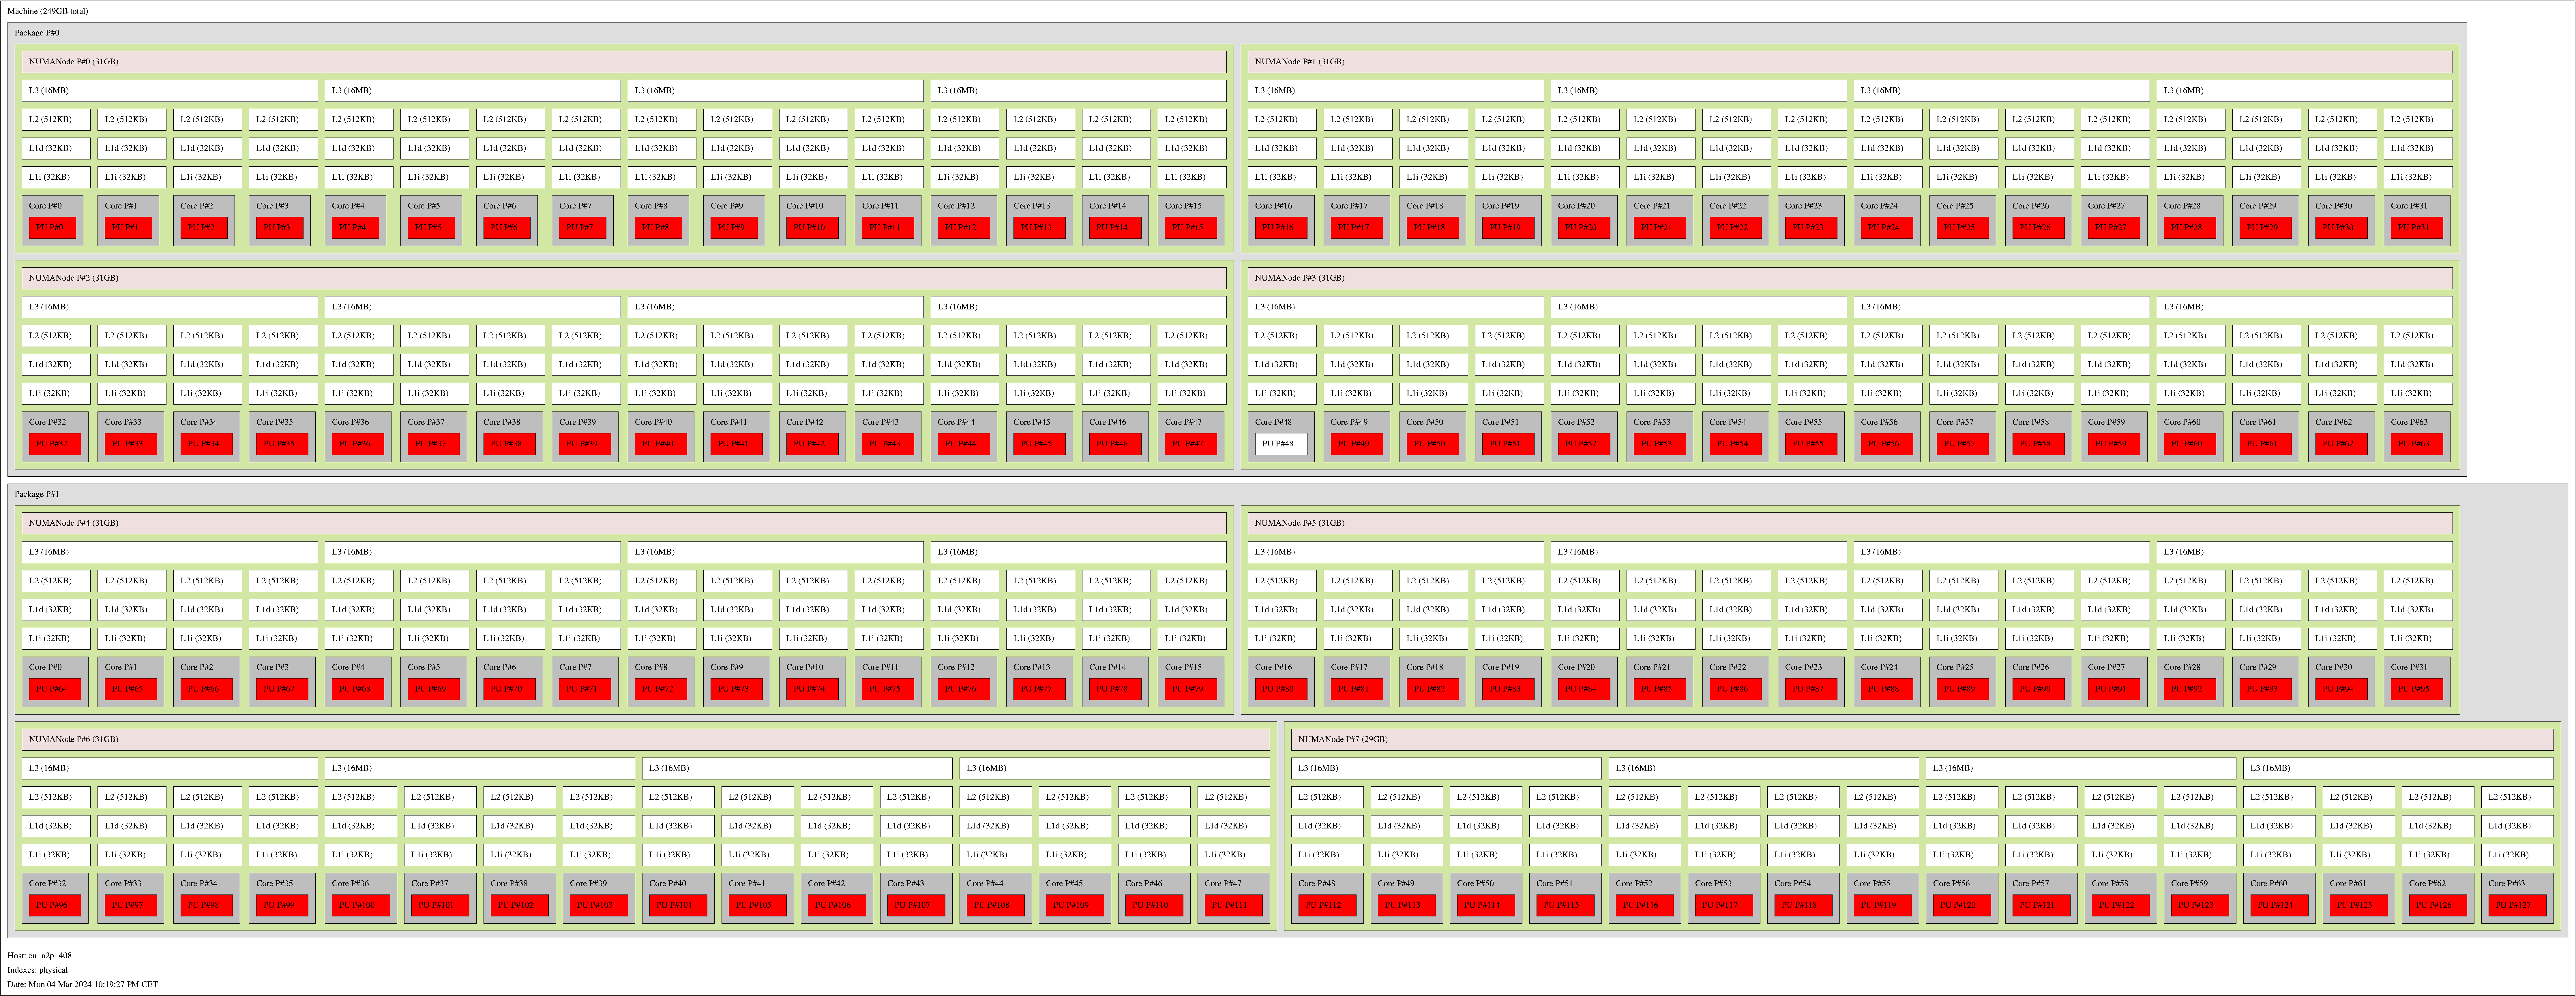
\includegraphics[width=\textwidth]{Images/AMD_EPYC_7H12.pdf}
    \caption{Schematic of an Euler login node with an AMD EPYC 7H12 CPU.}
    \label{fig:memory_euler_7H12}
\end{figure}

\begin{figure}[H]
    \centering
    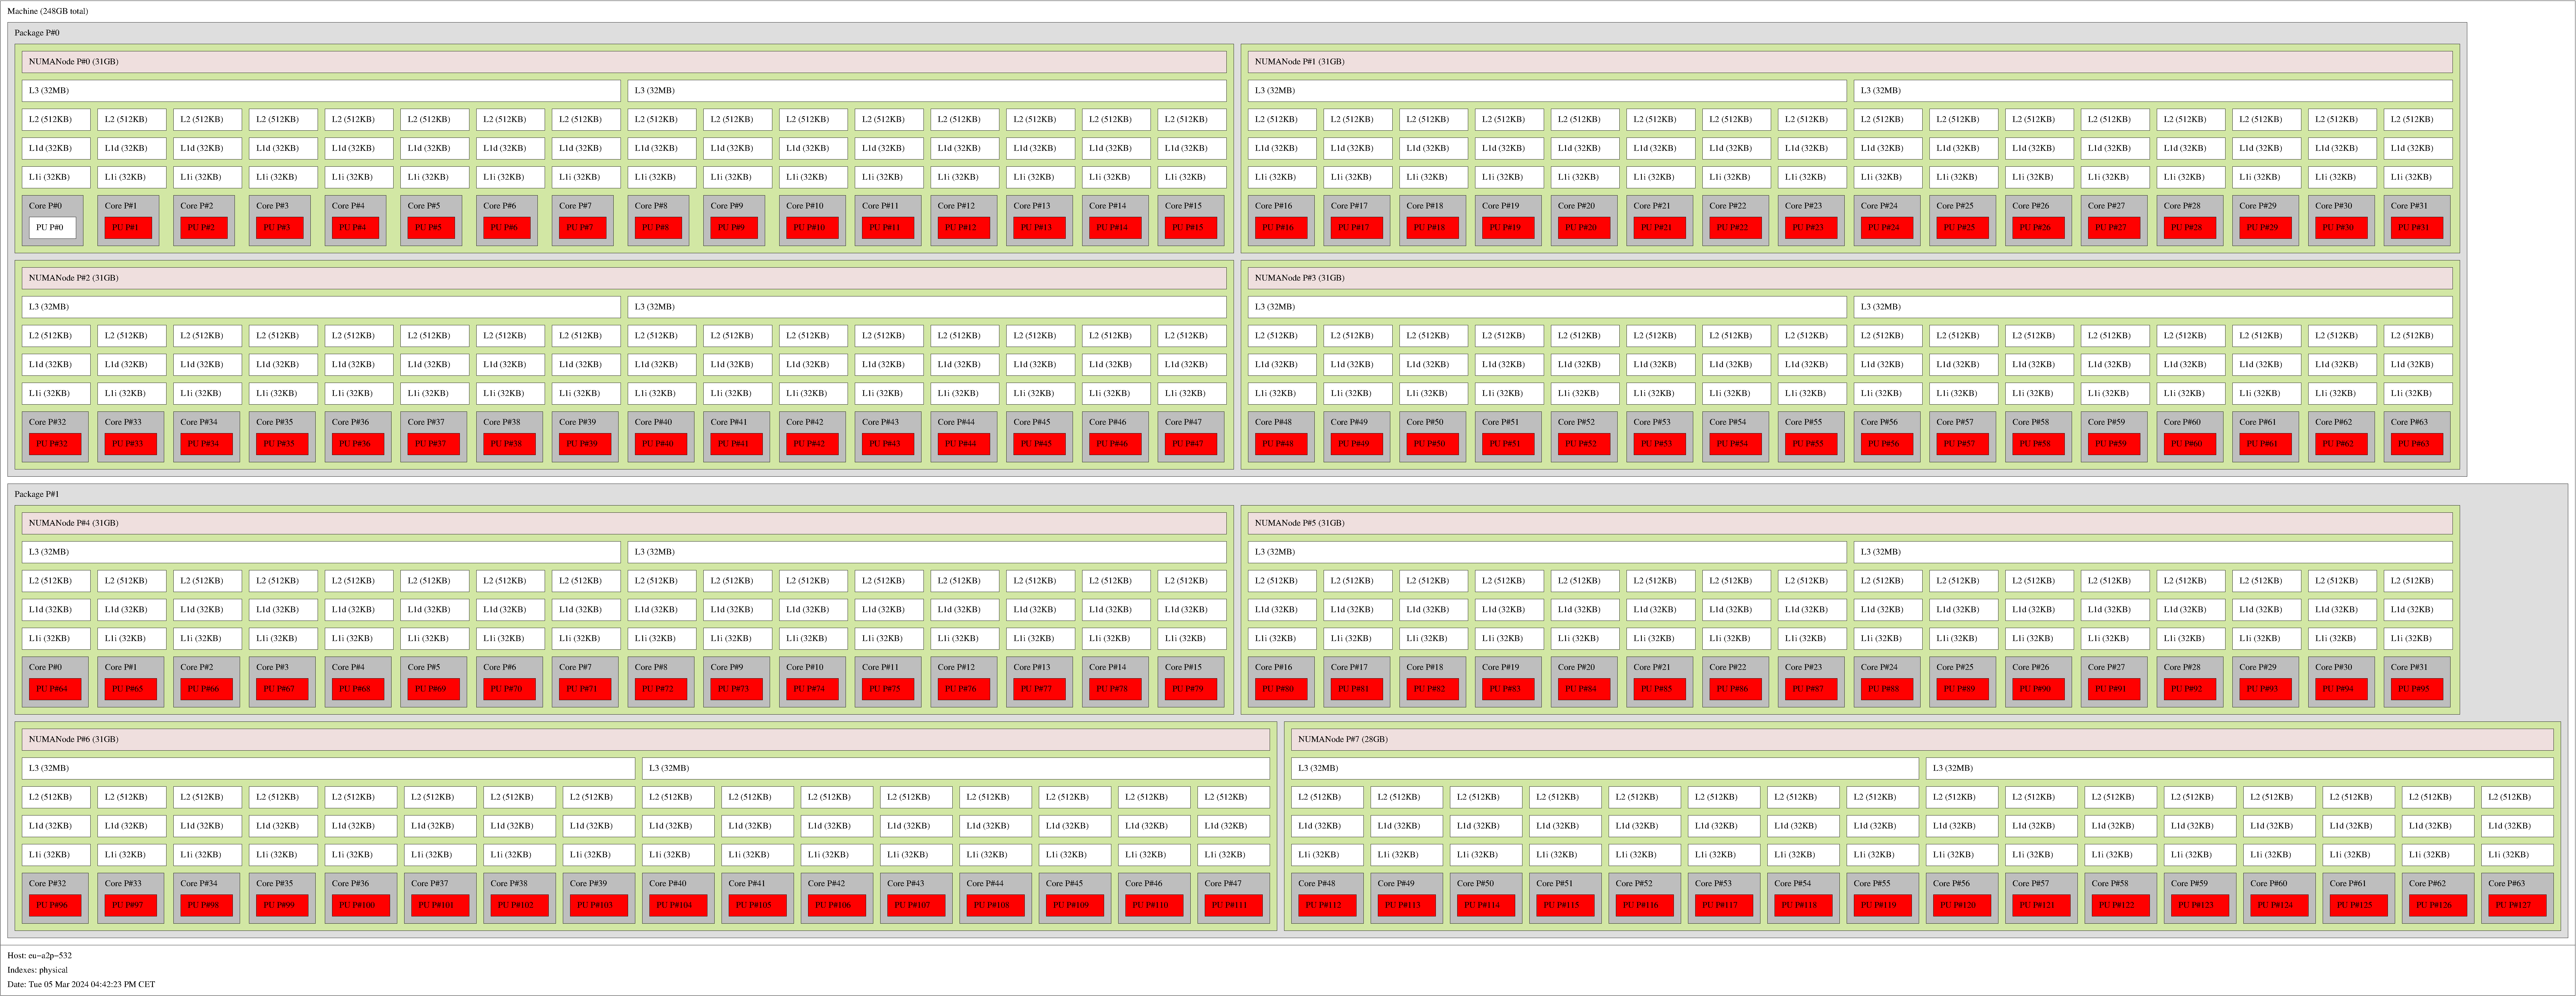
\includegraphics[width=\textwidth]{Images/AMD_EPYC_7763.pdf}
    \caption{Schematic of an Euler login node with an AMD EPYC 7763 CPU.}
    \label{fig:memory_euler_7763}
\end{figure}

\subsection{Bandwidth: STREAM benchmark}

For the STREAM benchmark we can use the provided file \texttt{stream.c}, where we need to adjust the STREAM\_ARRAY\_SIZE Parameter
in the C-file for our system. In particular our two systems are, the Euler VII Phase 1 with the AMD EPYC 7H12 CPU and for Euler VII Phase 2
with the AMD EPYC 7763 CPU. According to the \texttt{stream.c} file provided by "Dr. Bandwidth", we have to calculate the STREAM\_ARRAY\_SIZE
by considering the following two criteria.
\begin{enumerate}
    \item {The first criteria is that each array must be at least 4 times the size of the available cache memory. Note that it is important to considering
           from Figures \ref{fig:memory_euler_7H12} and \ref{fig:memory_euler_7763} only one node.}
    \item {The size should be large enough so that the 'timing calibration' output by the program is at least 20 clock-ticks. Furthermore, 
    according to \texttt{stream.c} most versions of Windows have a 10 millisecond timer granularity. This assumption doesn't hold true for the euler
    cluster!}
\end{enumerate}
Retrieving the results from the previous task, namely Table\ref{tab:summary_memory}, we can see that we get for Euler VII Phase 1 the following results:
\begin{align*}
    \bar{L1} &= 4 \cdot 32 KB = 128 KB \\
    \bar{L2} &= 4 \cdot 512 KB = 2.048 MB \\
    \bar{L3} &= 4 \cdot 16 MB = 64 MB .
\end{align*}
While we would get for Euler VII Phase 2 these results:
\begin{align*}
    \bar{L1} &= 4 \cdot 32 KB = 128 KB \\
    \bar{L2} &= 4 \cdot 512 KB = 2.048 MB \\
    \bar{L3} &= 4 \cdot 32 MB = 128 MB .
\end{align*}
By respecting the second criteria the chosen parameter values can be extracted from Figure \ref{fig:slurm_euler_1} and \ref{fig:slurm_euler_2}.
\begin{figure}[H]
    \centering
    \VerbatimInput{Data_Output/slurm-euler_phase_1.txt}
    \caption{STREAM benchmark result for Euler VII Phase 1}
    \label{fig:slurm_euler_1}
\end{figure}
As done in the exercise sheet for a rough estimate we can assume for the Euler VII Phase 1 a maximum bandwidth $b_{STREAM}$ = 17 GB/s, which corresponds to the scale function.
Same thing is possible where the Euler VII Phase 2, where we can retrieve from Figure \ref{fig:slurm_euler_2} a maximum bandwidth value of $b_{STREAM}$ = 27 GB/s, which corresponds
to the add function.
\begin{figure}[H]
    \centering
    {\fontsize{8}{10}\selectfont
    \VerbatimInput{Data_Output/slurm-euler_phase_2.txt}}
    \caption{STREAM benchmark result for Euler VII Phase 2}
    \label{fig:slurm_euler_2}
\end{figure}

\subsection{Performance model: A simple roofline model}

As a result, the last question is to answer, at what operational intensity is a kernel or application memory/compute-bound? To 
answer this question the provided paper by Williams et al. demonstrates the roofline model, which can be described as a 
visual performance model, that can help in order to optimize code and software for floating point computations. Furthermore, 
the proposed model combines three important computer metrics which were already computed in the prior tasks. Parameters included
are, the floating point performance, the operational intensity and the memory performance. The resulting 2D graph then consists
of the following two parts:
\begin{enumerate}
    \item Horizontal line: represents the peak floating point performance of the core.
    \item Linear line: represents the peak memory bandwidth.
\end{enumerate}
Moreover, the intersection between the two lines results in a point, which describes the limits for the underlying 
system. As a result to determine at what operational intensity a kernel or application is memory-bound or compute-bound,
we have to look at where the performance of the kernel intersects (the described critical point) with the memory
bandwidth line on the graph. Hence, on one hand, if the kernel's performance is below this line, it's liekly memory-bound. 
On the other hand, if it's above the line it's compute-bound.

\begin{figure}[H]
    \centering
    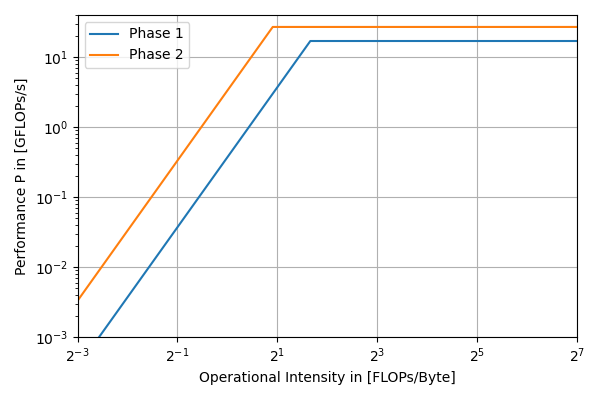
\includegraphics[width=\textwidth]{Images/performance.png}
    \caption{Simple roofline model for a single Euler VII Phase 1 and Phase 2 core.}
    \label{fig:performance}
\end{figure}
As a result if we look at Figure \ref{fig:performance}, it is clear that the kernel or application is memory-bound at 
operational intensity I values below 3.2 and 1.9 for the Euler VII Phase 1 and 2 core respectively. If values are above
this critical point the kernel and application is compute-bound. \\ \\
Note that on the next page the solution for the Project 1b starts.

\newpage
\section{Auto-vectorization [10 points]}

\subsection{Why is it important for data structures to be aligned?}
From the Intel Compiler Guide \cite{autovectorization} we can extract the information that data 
structure alignment is the adjustment of any data object with relation to other objects. This alignment 
offers the opportunity to speed up memory access. As a result, it's important to know that misaligned memory accesss 
can result in performance losses. Hence data structures have to bused in order to store data on a computer so that it can be used efficiently!

\subsection{What are some obstacles that can prevent automatic vectorization by the compiler?}
Again in the Intel Compiler Guide \cite{autovectorization}, it's mentioned that in the following cases the compiler decides that 
vectorization would not be worthwhile.
\begin{itemize}
    \item {\textbf{Non-contiguous memory access:} if 4 consecutive integers, floats, or 2 consecutive doubles are not adjacent, 
    they must be loaded separately using multiple instructions, which is considerably less efficient.}
    \item {\textbf{Data dependencies:} Vectorization results in changes in the order of operations within a loop. This is only possible, 
    if this change of order doesn't change the results of the calculation.}
\end{itemize}

\subsection{Is there a way to help the compiler to vectorize and how?}
When there is insufficient information for the compiler to decide to vectorize a loop, the following ways presents a solution 
how the compiler is able to vectorize a given problem with additional information \cite{autovectorization}.
\begin{itemize}
    \item {\textbf{Pragmas}}
    \item {\textbf{Keywords:} The restrict keword for instance can help the compiler to asswert that the memory referenced by a pointer 
    is not aliased.}
    \item {\textbf{Options/Switches:} enables different levels of optimizations to achieve automatic vectorization.}
\end{itemize}

\subsection{Which loop optimizations are performed by the compiler to vectorize and pipeline loops?}
These loop optimizations are typically performed by the compiler:
\begin{itemize}
    \item {\textbf{Stop-mining and Cleanup:} Strip-mining also known as loop sectioning is a loop transformation technique for enabling SIMD-encoding 
    of loops. This improves memory performance. Another possibility in this context is loop blocking.}
    \item {\textbf{Loop Interchange and Subscripts with Matrix Multiply:} This improves memory the memory access patterns. The result of this method can be 
    seen especially in the next task to optimize the DGEMM.}
\end{itemize}

\subsection{What can be done if automatic vectorization by the compiler fails or is sub-optimal?}
There are different ways to solve this problem, as illustrated in the following points.
\begin{itemize}
    \item {\textbf{Manual Vectorization:} As done in the following DGEMM example code can be rewritten to explicitly use vectorization instructions.}
    \item {\textbf{Loop Unrolling:} This can also be done manually and reduce loop overhead.}
    \item {\textbf{Pragma Directives:} Further pramga directives such as \#pragma omp simd.}
    \item {\textbf{Keywords:} Additional keywords like restrict.}
    \item {\textbf{Compiler Flags:} Additional or more aggresive compiler optimization flags can resolve this problem.}
    \item {\textbf{Profiling:} Analysis of the generated assembly code to identify bottlenecks and areas of improvement.}
    \item {\textbf{Software Pipelining:} This technique allows overlapping of loop iterations and improve vectorization.}
\end{itemize}
Which one of the mentioned approaches actually helps, depends ont the specific code and architecture. It could be seen from the next example the optimization of the DGEMM problem. 
It becomes evident that not all of the mentioned optimization techniques to assure vectorization help.

\section{Matrix multiplication optimization [30 points]}
The goal of this task is to optimize the naive matrix multiplication through replacing it with a 
blocking optimization. Also for further optimization its performance, we should consider various
additional strategies. In this part of the report I will present the evolution of how I reached 
better results through trying out different optimization strategies.
\newline
I started off by looking at the initial output first, without any optimization and only the comparison between 
the DGEMM (Double Precision GEneral Matrix Multiplication) implementation of the BLAS library, which is highly 
optimized and the naive matrix multiplication. The result can be seen in the Figure \ref{fig:no_opt}

\begin{figure}[H]
    \centering
    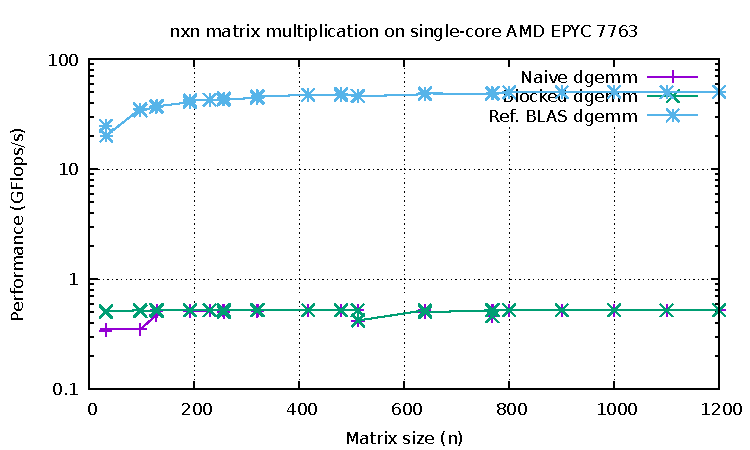
\includegraphics[width=\textwidth]{Images/timing_without_opt.pdf}
    \caption{Results of the DGEMM without any optimization.}
    \label{fig:no_opt}
\end{figure}

From this image, it's evident, as described in the exercise sheet that there is a huge optimization potential with the 
goal to come as close as possible to the BLAS implementation. First step I did to improve the results was to add optimization 
flags to push the results of the naive approach a little closer.
\begin{figure}[H]
    \centering
    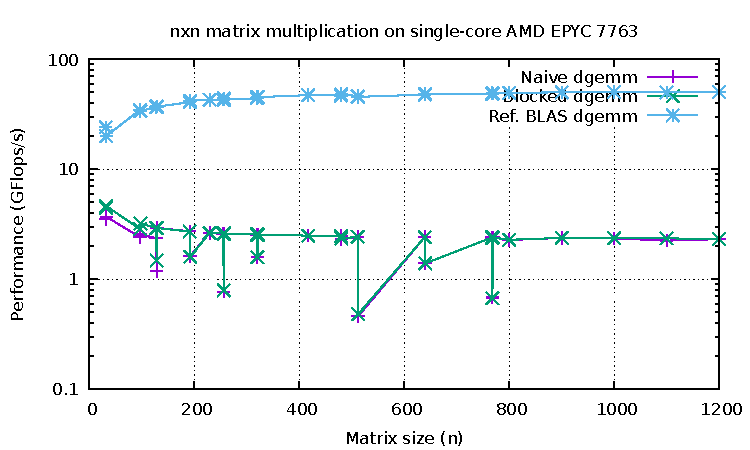
\includegraphics[width=\textwidth]{Images/timing_compiler_opt.pdf}
    \caption{Results of the DGEMM with compiler optimization.}
    \label{fig:compiler_opt}
\end{figure}
As a result, Figure \ref{fig:compiler_opt} shows that just by adding some compiler flags can improve the results dramastically.
I will briefly summarize the utilized compiler flags:
\begin{itemize}
    \item {\textbf{-03}: This flag represents the optimization level, where I used an aggressive approach that even outperforms
            -Ofast.} 
    \item \textbf{-march=native}: This gives the compiler the instruction to generate code for the host machine's architecture.
    \item \textbf{-funroll-loops}: This compiler flag enables loop unrolling.
\end{itemize}
It becomes evident from Figure \ref{fig:compiler_opt} that only these few flags have a huge effect on the overall performance of 
the DGEMM task. A compiler optimization guide provided specifically for the used AMD EPYC processor series offers more insights 
in how to tune a GNU compiler for even more optimized results \cite{compiler_opt_guide}, \cite{compiler_best_practice}. In \cite{compiler_best_practice} 
the suggested compiler flags for a GNU compiler area as follows:
\begin{align*}
    OPT &= -O3 -march=znver1 -mtune=znver1 -mfma \\
        &\quad -mavx2 -m3dnow -fomit-frame-pointer
\end{align*}
This should lead to a god optimized result and in the end should generate optimal code for the 
AMD EPYC processor \cite{compiler_best_practice}. Unfortunatelly this wasn't the case for me, 
I think it is due to \#pragma intrinsicts that should have been placed more properly to make use of 
SIMD. That's why I used the following compiler flags, as already presented:
\begin{align*}
    OPT = -O3 -march=native -funroll-loops
\end{align*}
Also to mention just a few, I tried other compiler flags such as -ftree-vectorize -fopt-info-vec to further 
optimize DGEMM, but couldn't reach better results. A list of all possible compiler intrinsics for the underlying 
AMD EPYC processor can be found on Microsoft's webpage \cite{intrisic_list}.
\newline
In the next approach, since in the exercise sheet it was stated that the provided template uses the column major order storage 
scheme, I looked at the naive code closer and found that the loop hierarchy could be handled better. Through changing it I reached 
the following results, illustrated in Figure \ref{fig:naive}. Note that all compiler optimization described from before are 
utilized for all the following explanations.
\begin{figure}[H]
    \centering
    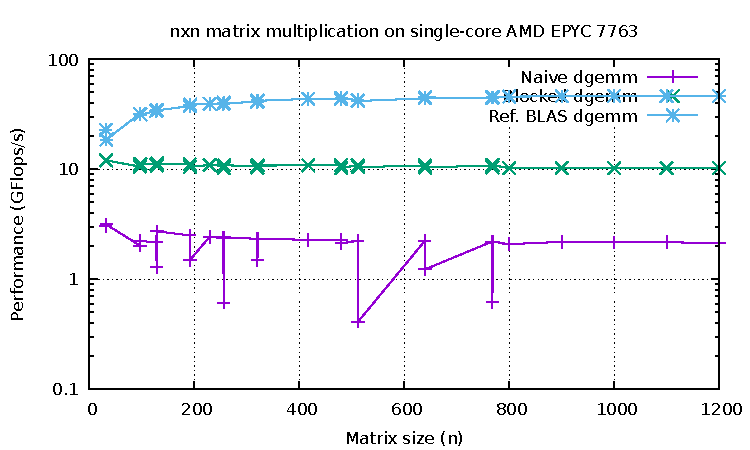
\includegraphics[width=\textwidth]{Images/timing_NAIVE.pdf}
    \caption{Results of the DGEMM with a loop rearrangement.}
    \label{fig:naive}
\end{figure}
From the image it's evident that rearranging the order of the loops has a huge impact on the overall performance since we can utilize 
a unity stride in a better way, as explained in the previous chapter where the concept of vectorization was discussed. Note that the underlying 
output files can be found in the Appendix of this chapter. From 
Figure \ref{fig:best} we can see that the average percentage of the peak performance is around 27,38\%. In comparison the so far 
best possible result, the BLAS library, has according to Figure \ref{fig:blas} an average percentage of the peak performance around 102,02\%. 
Unfortunatelly, this was already my best result I could achieve.
\newline
Nevertheless I will present further optimization trials. Since the main task was to implement a blocked matrix DGEMM approach, I briefly 
want to adress this task as well. The resulting code for this task can be found in the \texttt{dgemm-blocked.c}, where both versions, 
my optimized naive approach as well as the tiled matrix DGEMM are available. From the exercise sheet it becomes evident that for this approach 
we need a block size to split the problem up and this size actually depends on the underlying processor architecture. From previous tasks 
we know that we want to store frequently used data inside the L1 cache, as close as possible to the CPU. The memory capacity of the L1 
cache for the AMD EPYC 7763 processor is 32KB, we can utilize the conversion that 1KB = 2024 Bytes and get in the end the following result
for an upper bound of the block size:
\begin{align*}
    s \leq \sqrt{\frac{32 \cdot 1024}{3 \cdot 8}} = 36 
\end{align*}
The product of $32 \cdot 1024$ has to be divided through $3 \cdot 8$ this is the case because the size of a double precision floating point 
is 8 Bytes. Also, as stated and explained in the exercise sheet s should be as large as possible to gain best results so in this case, 
the best result for the matrix blocking should be with a blocking size of 36. But since this is only a theoretical upper bound there is still 
some adjustment necessary. In my case, as evident from Figure \ref{fig:blocked}, I got the best results with a block size value of 26 instead of 36.
\newline
Initially, I had an average percentage of the peak performance around 22\%. Through further pragma directives I was able to tweak it at least up 
to a value of 24,66\%. The most important one is \#pragma unroll which tells the compiler to unroll the following loop. Another used pragma directive 
is \#pragma omp atomic, which helped eventhough there was no multithreading involved. For some strange reason also the second used pragma directive 
is just for parallel computation, but it still improved my results a bit, which doesn't make any sense to be honest. \#pragma omp parallel for collapse(2)
enables parallelization across the following two loop dimensions for improved performance in a parallel computing environment. Also I want to mention 
another rather strange observation if the block size was defined with a preprocessor directive, more specifically the macro named BLOCK\_SIZE, instead of
initializing it with an integer, the performance dropped rapidly from 24\% to 10\%. Hence I stayed with the implementation provided in the code.
\newline
To summarize my result briefly, eventhough I tried out all mentioned optimization techniques and did even further investigation I wasn't able 
to tweak the tiled matrix multiplication to a better result than the naive approach.

\newpage
\subsection{Appendix}% Add to table of contents without numbering
The following Figures \ref{fig:basic}, \ref{fig:blocked}, \ref{fig:best} and \ref{fig:blas} are the outputted results for the AMD 
EPYC 7763 processor on the Euler cluster.

\begin{figure}[H]
    \centering
    {\fontsize{8}{10}\selectfont
    \VerbatimInput{Data_Output/timing_basic_dgemm.txt}}
    \caption{This is the result without any optimization of the basic/naive DGEMM.}
    \label{fig:basic}
\end{figure}

\begin{figure}[H]
    \centering
    {\fontsize{8}{10}\selectfont
    \VerbatimInput{Data_Output/timing_blocked_dgemm_BLOCKED.txt}}
    \caption{This is the result of the implemented and even more optimized matrix blocking/tiling approach.}
    \label{fig:blocked}
\end{figure}

\begin{figure}[H]
    \centering
    {\fontsize{8}{10}\selectfont
    \VerbatimInput{Data_Output/timing_blocked_dgemm_NAIVE.txt}}
    \caption{This is the result of the fine tuned and optimized naive DGEMM.}
    \label{fig:best}
\end{figure}

\begin{figure}[H]
    \centering
    {\fontsize{8}{10}\selectfont
    \VerbatimInput{Data_Output/timing_blas_dgemm.txt}}
    \caption{This is the result of the the BLAS library for the DGEMM task.}
    \label{fig:blas}
\end{figure}

\newpage
% \section*{References}  % Use \section* to prevent section number
\addcontentsline{toc}{section}{References}  % Add to table of contents without numbering

\bibliographystyle{unsrt}
\bibliography{library}

\end{document}
